% ch5.tex
% This work is licensed under the Creative Commons Attribution-Noncommercial-Share Alike 3.0 New Zealand License.
% To view a copy of this license, visit http://creativecommons.org/licenses/by-nc-sa/3.0/nz
% or send a letter to Creative Commons, 171 Second Street, Suite 300, San Francisco, California, 94105, USA.


\chapter{Una y otra vez}\label{ch:againandagain}

No hay nada peor que tener que hacer lo mismo una y otra vez.  Hay una razón por la que tus padres te dicen que cuentes ovejas para que te duermas, y no tiene nada que ver con el sorprendente poder para inducir al sueño de los mamíferos lanosos. Lo que importa es el hecho de que repetir algo sin parar es aburrido, y a tu cerebro le debería resultar más fácil dormirse si no está pensando en cosas interesantes.
\par
Particularmente a los programadores tampoco les gusta repetirse. También les da el sueño.  Esta es una buena razón por la que todos los lenguajes de programación tienen lo que se llama un \textbf{for-loop}\footnote{En inglés `for' significa `para' y `loop' signica `giro' o `bucle'}\index{for - bucle}. Por ejemplo, para imprimir 5 veces la palabra hola en Python, \emph{podrías} escribir lo siguiente:

\begin{listing}
\begin{verbatim}
>>> print("hola")
hola
>>> print("hola")
hola
>>> print("hola")
hola
>>> print("hola")
hola
>>> print("hola")
hola
\end{verbatim}
\end{listing}

Lo que es$\ldots$ bastante aburrido.

O podrías utilizar un bucle for-loop (nota: hay 4 espacios en la segunda línea antes de la sentencia print---Los hemos resaltado utilizando @ para que puedas ver donde están):

\begin{listingignore}
\begin{verbatim}
>>> for x in range(0, 5):
... @@@@print('hola')
... 
hola
hola
hola
hola
hola
\end{verbatim}
\end{listingignore}

La función \code{range}\footnote{En inglés `range' significa `rango'}\index{funciones!range} permite crear de forma rápida y sencilla una lista de números que comienza en el primero y finaliza antes del último. Por ejemplo:

\begin{listing}
\begin{verbatim}
>>> print(list(range(10, 20)))
[10, 11, 12, 13, 14, 15, 16, 17, 18, 19]
\end{verbatim}
\end{listing}

Por eso, en el caso del for-loop, lo que el código `\code{for x in range(0, 5)}' le está diciendo a Python es que cree una lista de números [0, 1, 2, 3, 4] y que luego, para cada número---de uno en uno---, lo guarde en la variable \code{x}. Por eso podríamos usar la variable x en la sentencia que imprime si así lo quisieramos:

\begin{listing}
\begin{verbatim}
>>> for x in range(0, 5):
...     print('hola %s' % x)
hola 0
hola 1
hola 2
hola 3
hola 4
\end{verbatim}
\end{listing}

Si no lo hiciéramos con la sentencia for-loop, el código que habría que escribir sería algo así:

\begin{listing}
\begin{verbatim}
x = 0
print('hola %s' % x)
x = 1
print('hola %s' % x)
x = 2
print('hola %s' % x)
x = 3
print('hola %s' % x)
x = 4
print('hola %s' % x)
\end{verbatim}
\end{listing}

Así que la sentencia for, que nos permite hacer un bucle, nos ha ahorrado tener que teclear 8 líneas extra de código.  Esto es muy útil, puesto que un programador normal, cuando tiene que teclear, es más perezoso que un hipopótamo en un día de calor. Los buenos programadores odian tener que hacer las cosas más de una vez, por eso la sentencia for es una de las más útiles en cualquier lenguaje de programación.

\fbox{\colorbox{PaleBlue}{\parbox{.75\linewidth} {
\subsection*{¡¡¡AVISO!!!}

Si has intentado teclear los ejemplos anteriores sobre la marcha, podría ser que Python te haya mostrado un extraño mensaje de error cuando introdujiste el código dentro del for-loop.  Si fue así se parecería a esto:

\begin{listing}
IndentationError: expected an indented block\footnote{Los mensajes de error de la consola de Python suelen ser en inglés, en este caso significa que hay error de indentación y que se espera un bloque de código indentado}
\end{listing}

Si ves un error como este, significa que te ha faltado teclear los espacios de la segunda línea.  En Python los espacios son muy importantes (o un espacio normal o un tabulador).  Hablaremos sobre ellos enseguida$\ldots$
}}}
\linebreak
\par
En realidad no tenemos que utilizar la función \code{range}, podemos utilizar las listas que hayamos creado.  Como por ejemplo, la lista de la compra que creamos en el último capítulo:

\begin{listing}
\begin{verbatim}
>>> lista_de_la_compra = [ 'huevos', 'leche', 'queso', 'apio', 
... 'manteca de cacahuete', 'levadura' ]
>>> for i in lista_de_la_compra:
...     print(i)
huevos
leche
queso
apio
manteca de cacahuete
levadura
\end{verbatim}
\end{listing}

El código anterior es una forma de decir, ``para cada elemento en la lista, almacena el valor en la variable `i' y luego imprime el contenido de esa variable''.  Si, como antes, no utilizásemos el bucle for-loop, tendríamos que haber hecho algo así:

\begin{listing}
\begin{verbatim}
>>> lista_de_la_compra = [ 'huevos', 'leche', 'queso', 'apio', 
... 'manteca de cacahuete', 'levadura' ]
>>> print(lista_de_la_compra[0])
huevos
>>> print(lista_de_la_compra[1])
leche
>>> print(lista_de_la_compra[2])
queso
>>> print(lista_de_la_compra[3])
apio
>>> print(lista_de_la_compra[4])
manteca de cacahuete
>>> print(lista_de_la_compra[5])
levadura
\end{verbatim}
\end{listing}

Gracias al bucle nos hemos ahorrado tener que teclear un montón de código.

La figura~\ref{for} trata de explicar de forma gráfica el funcionamiento del bucle for. Python llega al bucle for y observa la lista. Lo primero que hace es iniciar un contador interno que nosotros no vemos nunca pero que a Python le vale para saber por dónde va ejecutando el bucle y cuándo tiene que terminar. Luego, antes de hacer ninguna sentencia del bloque interior lo siguiente que hace es comprobar que el contador no ha llegado al final de la lista. Esto lo hace incluso la primera vez. Ten en cuenta que la lista podría no tener ningún elemento (podría estar vacía). Si aún quedan elementos, el contador es menor que el número de elementos de la lista, entonces asigna a la variable que hemos dicho el elemento correspondiente de lista y ejecuta el bloque de la setencia for una vez. Finalizada la ejecución del bloque, incrementa en uno el contador y vuelve al comienzo a preguntar si el contador es menor que el número de elementos. Así se ejecuta, tantas veces como elementos haya en la lista. Cuando el contador ya no sea menor que los elementos de la lista el bucle for termina.

\begin{figure}
\begin{center}
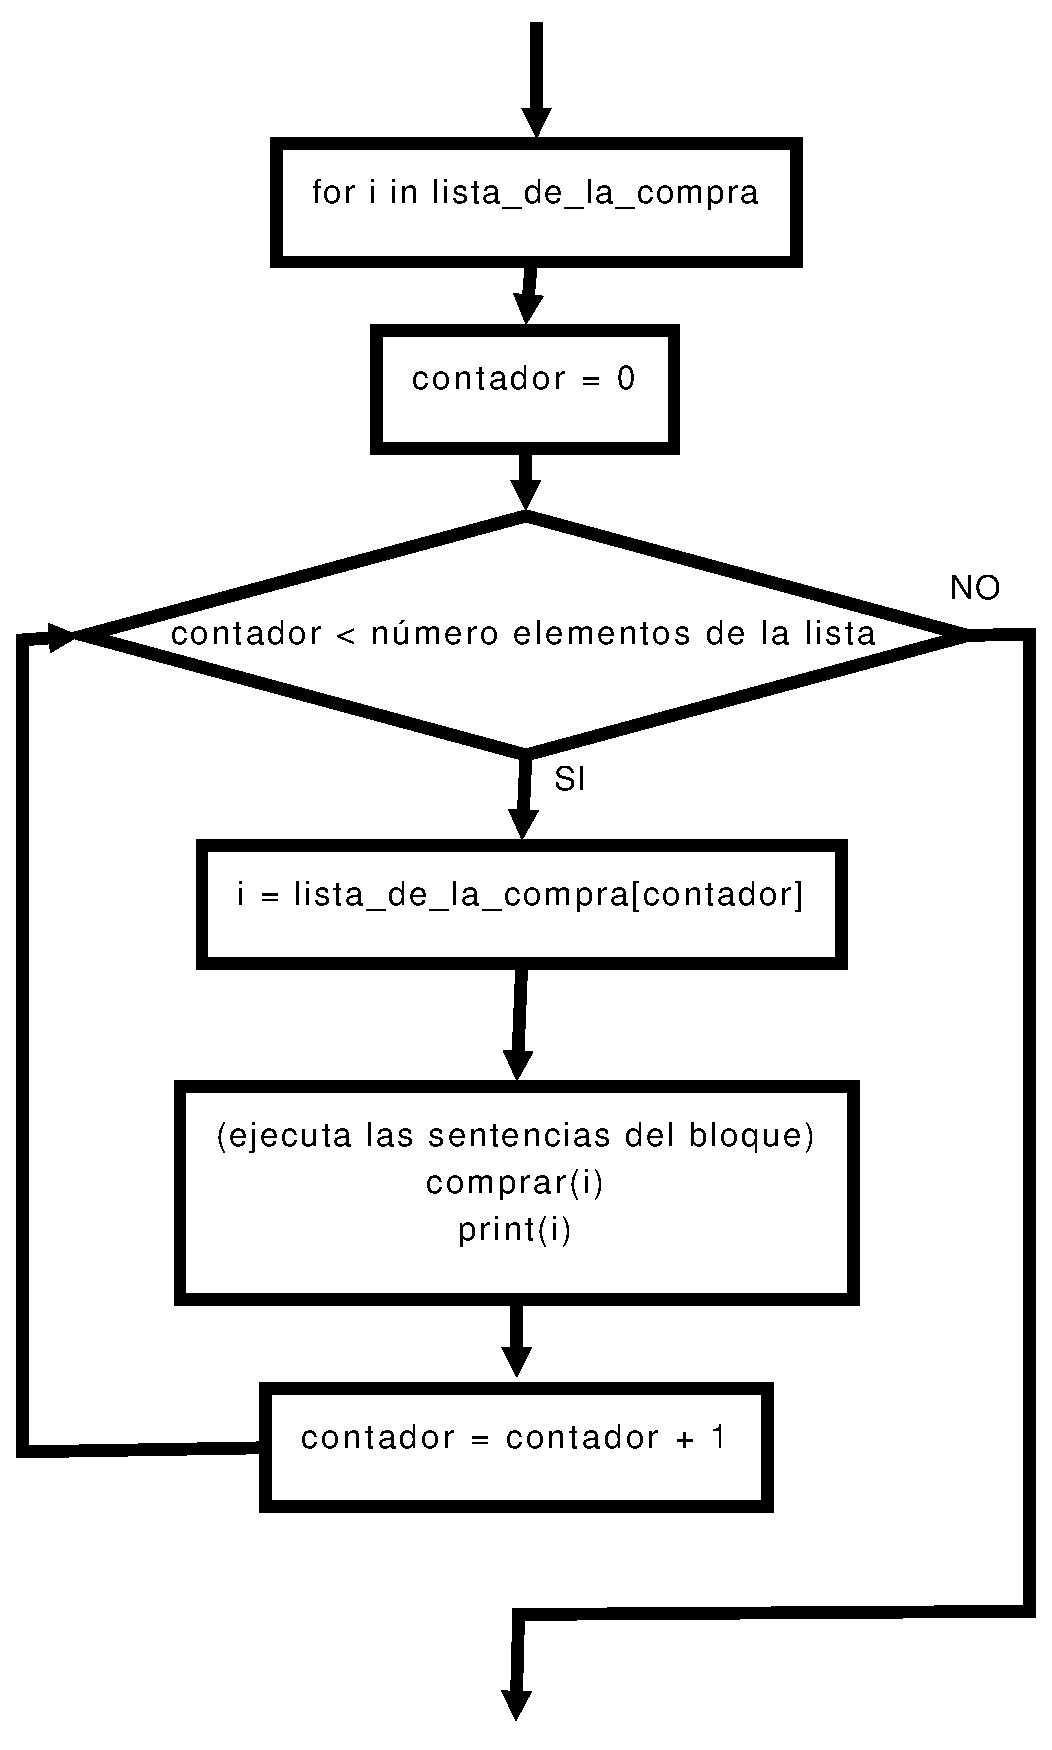
\includegraphics[width=90mm]{for.eps}
\end{center}
\caption{Dando vueltas en un bucle for.}\label{for}
\end{figure}

\section{¿Cuándo un bloque no es cuadrado?}\index{bloques de código}

Cuando es un bloque de código.
\par
\noindent
¿Y qué es lo que es un `bloque de código'?
\par
Un bloque de código es un conjunto de sentencias del programa que quieres que estén agrupadas.  Por ejemplo, en el bucle for-loop anterior, podría suceder que quisieras hacer algo más que imprimir los elementos de la lista.  Tal vez quisieras comprar cada elemento y luego imprimirlo.  Suponiendo que tuviéramos una función llamada `comprar', podríamos escribir el siguiente código:

\begin{listingignore}
\begin{verbatim}
>>> for i in lista_de_la_compra:
...     comprar(i)
...     print(i)
\end{verbatim}
\end{listingignore}

No te molestes en teclear el ejemplo anterior en la consola de Python---porque no tenemos ninguna función comprar y dará un mensaje de error si intentas ejecutarlo---únicamente nos sirve para demostrar el uso de un bloque de código de Python compuesto por 2 sentencias:

\begin{listingignore}
\begin{verbatim}
comprar(i)
print(i)
\end{verbatim}
\end{listingignore}

En Python, los espacios en blanco\index{espacio en blanco} resultado del tabulador (cuando pulsas la tecla tab) y del espacio (cuando pulsas la barra espaciadora) son \emph{muy} importantes.  El código que está en la misma posición queda agrupado para formar bloques.

\begin{listing}
\begin{verbatim}
    esto podría ser el bloque 1
    esto podría ser el bloque 1
    esto podría ser el bloque 1
	        esto podría ser el bloque 2
	        esto podría ser el bloque 2
	        esto podría ser el bloque 2
    esto aún sería el bloque 1
    esto aún sería el bloque 1
	        esto podría ser bloque 3
	        esto podría ser bloque 3
	            esto podría ser bloque 4
	            esto podría ser bloque 4
	            esto podría ser bloque 4
\end{verbatim}
\end{listing}

Pero debes ser consistente con los espacios.  Por ejemplo:

\begin{listingignore}
\begin{verbatim}
>>> for i in lista_de_la_compra:
...     comprar(i)
...       print(i)
\end{verbatim}
\end{listingignore}

La segunda línea (función \code{comprar(i)}) comienza con \textbf{4} espacios.  La tercera (función \code{print(i)}) comienza con \textbf{6} espacios.  Veamos de nuevo el código haciendo visibles los espacios (utilizando @ de nuevo):

\begin{listingignore}
\begin{verbatim}
>>> for i in lista_de_la_compra:
... @@@@comprar(i)
... @@@@@@print(i)
\end{verbatim}
\end{listingignore}

Esto provocaría un error.  Una vez comienzas a utilizar 4 espacios, debes seguir usándolos.  Y si quieres poner un bloque \emph{dentro} de otro bloque, necesitarás usar más de 4 espacios, los que sean, pero los mismos durante todo el bloque.
Es buena práctica de programación utilizar el doble de los espacios del bloque inicial, en este caso 8 (2 x 4) al comienzo de las líneas del bloque interno. 
\par
Así que si el primer bloque tiene 4 espacios (Lo volveremos a resaltar para que puedas verlos):

\begin{listing}
\begin{verbatim}
@@@@Aquí está mi primer bloque
@@@@Aquí está mi primer bloque
\end{verbatim}
\end{listing}

El segundo bloque (que está `dentro' del primero) necesitará más de 4 espacios, vamos a usar 8:

\begin{listing}
\begin{verbatim}
@@@@Aquí está mi primer bloque
@@@@Aquí está mi primer bloque
@@@@@@@@Aquí está mi segundo bloque
@@@@@@@@Aquí está mi segundo bloque
\end{verbatim}
\end{listing}

Y si quisiéramos un tercer bloque `dentro' del segundo necesitaríamos más de 8 espacios. Para mantener nuestro criterio utilizaríamos 12 (3 x 4): 

\begin{listing}
\begin{verbatim}
@@@@Aquí está mi primer bloque
@@@@Aquí está mi primer bloque
@@@@@@@@Aquí está mi segundo bloque
@@@@@@@@Aquí está mi segundo bloque
@@@@@@@@@@@@Aquí está mi tercer bloque
@@@@@@@@@@@@Aquí está mi tercer bloque
@@@@@@@@@@@@Aquí está mi tercer bloque
\end{verbatim}
\end{listing}

A Python le es indiferente el número de espacios que use cada bloque siempre que sean los mismos para cada línea de un bloque, y que los bloques internos a otros (anidados) tengan más espacios que aquél en el que se anidan. No obstante, es buena práctica utilizar siempre el mismo número de espacios en el código para cada nivel de bloque con el fin de que quede más claro al leerlo. Norlmamente, como ya hemos comentado, usaremos múltiplos del primer nivel para los bloques interiores.

¿Por qué queremos poner un bloque `dentro' de otro?  Normalmente hacemos esto cuando el segundo bloque depende de alguna manera del primero.  Tal y como pasa con nuestro bucle for-loop.  Si la línea con el código for es el primer bloque, entonces las sentencias que queremos que se ejecuten una y otra vez están en el segundo bloque---estas sentencias dependen del primer bloque para funcionar apropiadamente (el valor de la variable del bucle cambia cada vez).
Por último, conviene tener en cuenta que el primer bloque está formado por todo lo que está a su nivel de espacios o más espaciado dentro de él. Hasta que aparece otra línea al mismo nivel.
Para aclararlo, muestro un par de ejemplos pero esta vez con rayitas destacando los bloques:

\begin{listing}
\begin{verbatim}
+---esto podría ser el bloque 1
|   esto podría ser el bloque 1
|   esto podría ser el bloque 1
|   +---esto podría ser el bloque 2
|   |   esto podría ser el bloque 2
|   +---esto podría ser el bloque 2
|   esto aún sería el bloque 1
|   esto aún sería el bloque 1
|   +---esto podría ser bloque 3
|   |   esto podría ser bloque 3
|   +---esto podría ser bloque 3
|       +---esto podría ser bloque 4
|       |   esto podría ser bloque 4
+-------+---esto podría ser bloque 4
\end{verbatim}
\end{listing}


\begin{listing}
\begin{verbatim}
+---Aquí está mi primer bloque
|   Aquí está mi primer bloque
|   +---Aquí está mi segundo bloque
|   |   Aquí está mi segundo bloque
|   |   +---Aquí está mi tercer bloque
|   |   |   Aquí está mi tercer bloque
+---+---+---Aquí está mi tercer bloque
\end{verbatim}
\end{listing}

Cuando inicias un bloque en la consola, Python continúa el bloque hasta que pulsas la tecla Intro en una línea en blanco (mientras se teclea el bloque la consola mostrará 3 puntos al comienzo de la línea para mostrar que estás aún en un bloque.

Vamos a intentar algunos ejemplos de verdad.  Abre la consola de Python y teclea  lo siguiente (recuerda que debes pulsar la barra espaciadora 4 veces al comienzo de las líneas con las funciones print)

\begin{listing}
\begin{verbatim}
>>> milista = [ 'a', 'b', 'c' ]
>>> for i in milista:
...     print(i)
...     print(i)
...
a
a
b
b
c
c
\end{verbatim}
\end{listing}

Después del segundo print, pulsa la tecla Intro en la línea en blanco---esto sirve para decirle a la consola que quieres finalizar el bloque. Entonces se imprimirá cada elemento de la lista dos veces.
\par
\noindent
El siguiente ejemplo provocará que se muestre un mensaje de error:

\begin{listing}
\begin{verbatim}
>>> milista = [ 'a', 'b', 'c' ]
>>> for i in milista:
...     print(i)
...       print(i)
...
File “<stdin>”, line 3
  print(i)
  ^
IndentationError: unexpected indent
\end{verbatim}
\end{listing}

El segundo print tiene 6 espacios, no 4, lo que no le gusta a Python ya que espera que los espacios permanezcan iguales dentro del bloque.

\fbox{\colorbox{PaleBlue}{\parbox{.75\linewidth} {
\subsection*{RECUERDA}

Si inicias los bloques de código con 4 espacios debes continuar utilizando 4 espacios.  Si inicias los bloques con 2 espacios, debes continuar utilizando 2 espacios.  Te recomiendo utilizar 4 espacios porque es lo que suelen utilizar los programadores expertos en Python.

}}}

\par
A continuación muestro un ejemplo más complejo con 2 bloques de código:

\begin{listing}
\begin{verbatim}
>>> milista = [ 'a', 'b', 'c' ]
>>> for i in milista:
...     print(i)
...     for j in milista:
...         print(j)
...
\end{verbatim}
\end{listing}

\noindent

¿Dónde están los bloques en este código? y ¿Qué es lo que hace?
\par
\noindent
Hay \textbf{dos} bloques---el primero es parte del primer bucle for-loop:

\begin{listing}
\begin{verbatim}
>>> milista = [ 'a', 'b', 'c' ]
>>> for i in milista:
...     print(i)                #
...     for j in milista:       #-- estas líneas forman el PRIMER bloque
...         print(j)            #
...
\end{verbatim}
\end{listing}

El bloque número dos es la línea print del segundo bucle for-loop:

\begin{listing}
\begin{verbatim}
>>> milista = [ 'a', 'b', 'c' ]
>>> for i in milista:
...     print(i)
...     for j in milista:
...         print(j)               # esta línea forma el SEGUNDO bloque
...
\end{verbatim}
\end{listing}

¿Puedes tratar de pensar que es lo que hace este código?
\par
Imprimirá las tres letras de `milista', pero ¿cuántas veces?  Si miramos a cada línea, probablelmente lo descubramos. Sabemos que el primer bucle recorrerá cada uno de los elementos de la lista, y luego ejecutará las sentencias del bloque número 1. Por lo que imprimirá una letra, luego comenzará el segundo bucle. Este bucle también recorrerá cada uno de los elementos en la lista y luego ejecutará la sentencia del bloque 2.  Por eso lo que deberíamos ver al ejecutar el código es `a' seguido de `a', `b', `c', luego `b' seguido de `a', `b', `c', para terminar con `c' y luego seguido de `a', `b' y `c'.  Introduce el código en la consola de Python para verlo tú mismo:

\begin{listing}
\begin{verbatim}
>>> milista = [ 'a', 'b', 'c' ]
>>> for i in milista:
...     print(i)
...     for j in milista:
...         print(j)
... 
a
a
b
c
b
a
b
c
c
a
b
c
\end{verbatim}
\end{listing}

¿Qué te parece hacer algo más útil que imprimir letras?  ¿Recuerdas el cálculo que hicimos al comienzo del libro para conocer cuánto podrías ahorrar al final del año si ganases 5 euros haciendo tareas, 30 euros repartiendo periódicos y gastases 10 euros a la semana?
\par
\noindent
Era así:

\begin{listing}
\begin{verbatim}
>>> (5 + 30 - 10) * 52
\end{verbatim}
\end{listing}

\noindent
(Son 5 euros más 30 euros menos 10 euros multiplicados por 52 semanas al año).

Podría ser útil ver cómo se incrementarían tus ahorros a lo largo del año según se van produciendo, en lugar de conocer únicamente lo que tendrás al finalizar.  Podemos hacerlo con un bucle for.  Pero primero tenemos que guardar estos números en variables:

\begin{listing}
\begin{verbatim}
>>> tareas = 5
>>> reparto = 30
>>> gastos = 10
\end{verbatim}
\end{listing}

Podemos ejecutar el cálculo original utilizando las variables:

\begin{listing}
\begin{verbatim}
>>> (tareas + reparto - gastos) * 52
1300
\end{verbatim}
\end{listing}

O podemos ver los ahorros incrementándose a lo largo del año. Para ello creamos otra variable y usamos un bucle:

\begin{listing}
\begin{verbatim}
1. >>> ahorros = 0
2. >>> for semana in range(1, 53):
3. ...     ahorros = ahorros + tareas + reparto - gastos
4. ...     print('Semana %s = %s' % (semana, ahorros))
5. ...
\end{verbatim}
\end{listing}

En la línea 1 la variable `ahorros' se inicia con el valor 0 (porque no hemos ahorrado nada aún).\\
La línea 2 prepara el bucle for que ejecutará todos las sentencias del bloque (el bloque está compuesto de las líneas 3 y 4).  Cada vez que se ejecuta el bucle la variable `semana' contiene el siguiente número en el rango que va de 1 a 52. Lo que significa que el bucle se ejecuta 52 veces, una por cada semana del año. todo ello gracias a la función range que genera una lista que contiene los números del 1 al 52.\\
La línea 3 es un poco más complicada.  Lo que queremos es que cada semana se sume lo que ahorramos con los ahorros que ya tenemos.   Piensa que la variable `ahorros' funciona como un banco.  Le añadimos el dinero que ganamos en nuestros trabajos y le quitamos los gastos y luego dejamos lo que queda en el banco.  Hablando en terminología informática, la línea 3 significa, ``suma los valores de las variables ahorros, tareas y  reparto, y réstale el valor de la variable gastos. El resultado asígnalo a la variable ahorros---que pierde así su valor original para guardar el nuevo valor''. En otras palabras, el símbolo igual (=) sirve en Python para decirle que ``haga todo lo que haya que hacer de cálculos a la derecha del igual y luego que lo guarde en la variable que está en la derecha''.\\ 
La línea 4 es una sentencia print un poco más complicada, imprime el número de semana y la cantidad ahorrada hasta la semana indicada.  Consulta la sección \emph{Trucos para las cadenas} en la página~\pageref{trickswithstrings}, si esta línea no tiene sentido para ti.  Por eso, el resultado si ejecutas este programa es el siguiente$\ldots$

\begin{listing}
\begin{verbatim}
Semana 1 = 25
Semana 2 = 50
Semana 3 = 75
Semana 4 = 100
Semana 5 = 125
Semana 6 = 150
Semana 7 = 175
Semana 8 = 200
Semana 9 = 225
Semana 10 = 250
Semana 11 = 275
Semana 12 = 300
Semana 13 = 325
Semana 14 = 350
Semana 15 = 375
\end{verbatim}
\end{listing}

$\ldots$y así hasta la semana 52.

\section{Saliendo de un bucle antes de tiempo}\index{palabras clave o reservadas!break}

La palabra reservada \textbf{break} se utiliza para parar la ejecución del bucle. Puedes utilizar la sentencia break dentro de un bucle for o while como en el siguiente ejemplo:

\begin{listing}
\begin{verbatim}
>>> edad = 10
>>> for x in range(1, 100):
...     print('contando %s' % x)
...     if x == edad:
...         print('fin de la cuenta')
...         break
\end{verbatim}
\end{listing}

Si la variable `edad' tuviera el valor 10, este código imprimiría:

\begin{listing}
\begin{verbatim}
contando 1
contando 2
contando 3
contando 4
contando 5
contando 6
contando 7
contando 8
contando 9
contando 10
fin de la cuenta
\end{verbatim}
\end{listing}

A pesar de que la cuenta del bucle for está prevista para 100 elementos. Existe una sentencia if que en cada paso del bucle for comprueba si la edad es igual a x. En el momento en que x coincide con edad (en este ejemplo es el número 10) se ejecuta el código de la sentencia if que es un print y un break. La sentencia break hace que se acabe el bucle for.


\section{Mientras hablamos sobre bucles$\ldots$}\index{while - bucle}

El bucle for no es la única clase de bucle que puede existir en Python. También existe el bucle while. Si en el bucle for se sabe exactamente el momento en que se finaliza, en el bucle while no se conoce necesariamente cuántas veces se ejecutará el mismo. Imagina una escalera de 20 escalones.  Sabes que puedes subirlos fácilmente.  Eso es un bucle for.

\begin{listing}
\begin{verbatim}
>>> for paso in range(0,20):
...     print(paso)
\end{verbatim}
\end{listing}

Ahora imagina una escalera que sube a lo largo de una montaña.  Te quedarías sin energía antes de alcanzar la cima.  O el tiempo podría empeorar forzándote a parar la escalada.  Esto es un bucle while\footnote{En inglés `while' significa `mientras'.}.

\begin{listingignore}
\begin{verbatim}
>>> paso = 0
>>> while paso < 10000:
...     print(paso)
...     if cansado:
...         break
...     elif maltiempo:
...         break
...     else:
...         paso = paso + 1
\end{verbatim}
\end{listingignore}

No te molestes en ejecutar el código del ejemplo anterior, porque no nos hemos preocupado de crear las variables \code{cansado} y \code{maltiempo}.  Pero demuestra lo fundamental de un bucle while.  El código del bloque se ejecutará una vez tras otra \emph{mientras} el valor de la variable \code{paso} sea menor que 10000 (paso $<$ 10000).  En el bloque, imprimimos el valor de \code{paso}, luego validamos si \code{cansado} or \code{maltiempo} tienen el valor verdadero (True). Si \code{cansado} es verdadero (tiene el valor True), entonces la sentencia \code{break} finaliza la ejecución del código del bucle (lo que sucede es que saltamos fuera del bucle a la siguiente línea de código que sigue al bloque inmediatamente después de él).  Si \code{maltiempo} es verdadero, también salimos del bucle.  Si no, entonces se suma \textbf{1} al valor de la variable \code{paso}, y se vuelve al comienzo, validándose de nuevo la condición de salida del bucle while (paso $<$ 10000).
\par
\noindent
Así que los pasos de un bucle while son fundamentalmente:

{\renewcommand{\labelitemi}{$\triangleright$}
\begin{itemize}
\item validar la condición que sigue a la palabra `while',
\item ejecutar el bloque,
\item volver al comienzo del bucle
\end{itemize}}

Si lo vemos, como en los ejemplos anteriores, con un diagrama, el bucle while funciona según se observa en la figura~\ref{while}.

\begin{figure}
\begin{center}
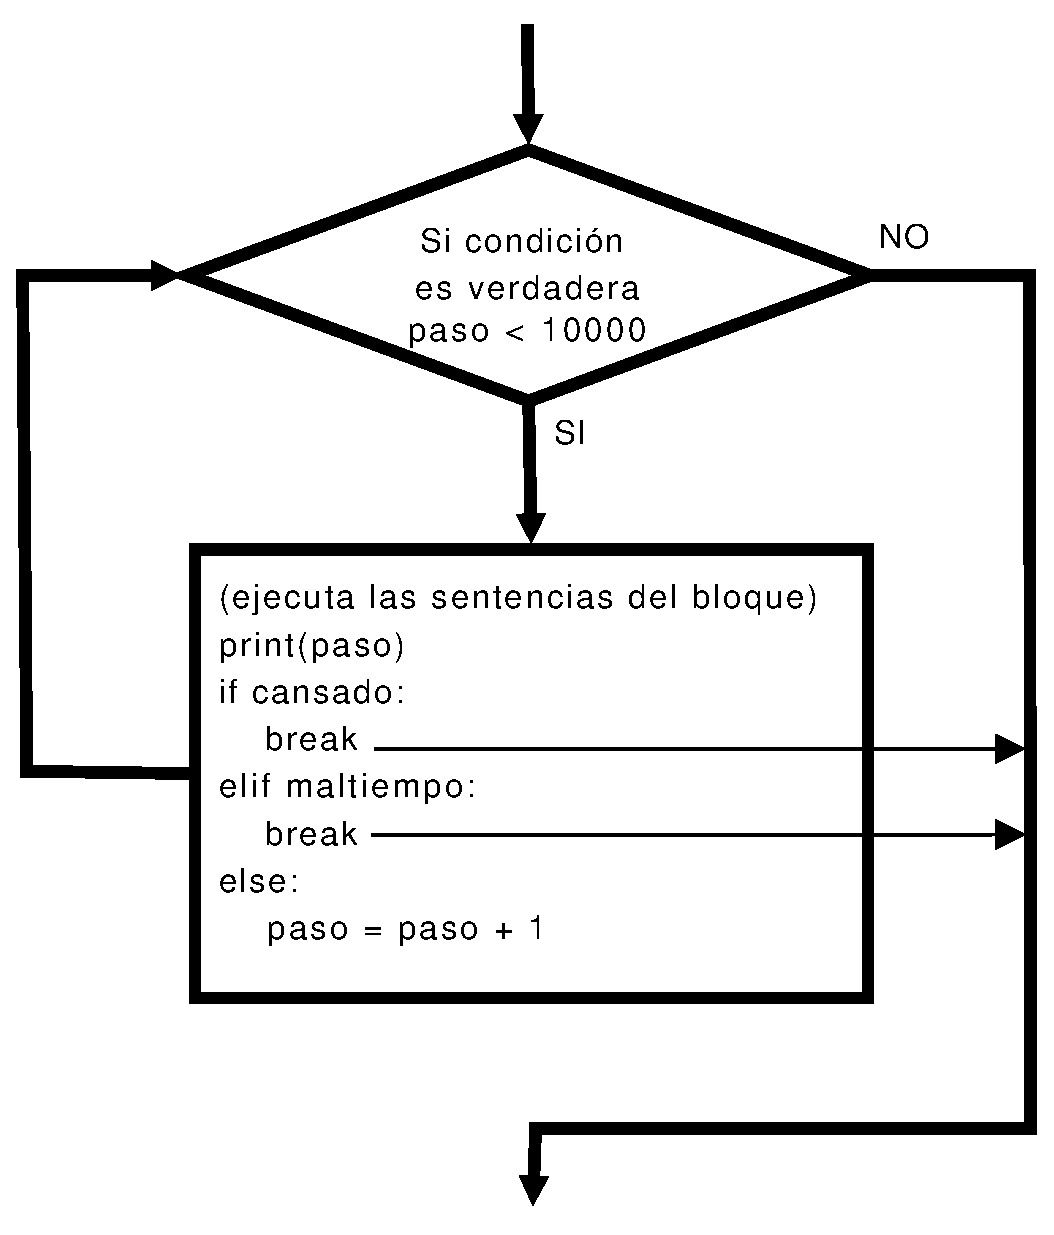
\includegraphics[width=80mm]{while.eps}
\end{center}
\caption{Dando vueltas en un bucle while.}\label{while}
\end{figure}

Es común que sea necesario crear bucles while que requieran más de una condición, por ejemplo un par de ellas:

\begin{listing}
\begin{verbatim}
>>> x = 45
>>> y = 80
>>> while x < 50 and y < 100:
...     x = x + 1
...     y = y + 1
...     print(x, y)
\end{verbatim}
\end{listing}

En este bucle creamos la variable \code{x} con el valor 45, y la variable \code{y} con el valor 80.  Hay dos condiciones que se chequean en el bucle: si \code{x} es menor que 50 y si \code{y} es menor que 100. Mientras ambas condiciones sean verdaderas, se ejecuta el bloque del código, sumando 1 a ambas variables y luego imprimiéndolas.  La salida en pantalla del código anterior es la siguiente:

\begin{listing}
\begin{verbatim}
46 81
47 82
48 83
49 84
50 85
\end{verbatim}
\end{listing}

Posiblemente ya seas capaz de figurarte porqué se imprimen estos números\footnote{Comenzamos contando en 45 en la variable \code{x} y en 80 en la variable \code{y}, y luego incrementamos (añadimos uno) a cada variable cada vez que se ejecuta una vuelta completa del bucle.  Las condiciones comprueban que \code{x} sea menor que 50 y que \code{y} sea menor que 100.  Después de cinco pasadas (sumando 1 a cada variable en cada pasada) el valor de x alcanza el número 50.  Ahora la primera condición (x $<$ 50) ya no es verdadera, por lo que Python finaliza el bucle.}

Otro uso habitual de un bucle while, es crear bucles casi eternos. O sea, un bucle que se ejecuta para siempre, o al menos hasta que sucede algo en el bloque de código interno que lo finaliza. Por ejemplo:

\begin{listingignore}
\begin{verbatim}
>>> while True:
...     Mucho código aquí
...     Mucho código aquí
...     Mucho código aquí
...     if alguna_condicion es verdadera:
...         break
\end{verbatim}
\end{listingignore}

La condición para el bucle while es `True'.  Por lo que siempre será verdadera y ejecutará contínuamente el código del bloque (así que el bucle es eterno o infinito). Solamente si la condición `alguna\_condicion' de la sentencia if es verdadera se ejecutará la sentencia break y se saldrá del bucle. Puedes ver un ejemplo mejor de este tipo de bucle en el Apéndice~\ref{app:afewpythonmodules} (en la sección sobre el módulo \code{random}), pero podrías querer esperar hasta que hayas leído el siguiente capítulo antes de echarle un vistazo.

\section{Cosas que puedes probar}

\emph{En este capítulo hemos visto como utilizar bucles para ejecutar tareas repetitivas.  Y hemos usado bloques de código dentro de los bucles para ejecutar las tareas que tenían que repetirse.}

\subsection*{Ejercicio 1}
¿Qué piensas que sucederá al ejecutar el siguiente código?

\begin{listing}
\begin{verbatim}
>>> for x in range(0, 20):
...     print('hola %s' % x)
...     if x < 9:
...         break
\end{verbatim}
\end{listing}

\subsection*{Ejercicio 2}
Cuando guardas dinero en un banco, ganas un interés.  El `interés' es el dinero que el banco te paga por dejarle que use tus ahorros---cada año te paga una pequeña cantidad de dinero dependiendo de cuanto tengas ahorrado.  Este pago normalmente se añade a tus ahorros en la cuenta del banco, con lo que pasa a formar parte de tus ahorros$\ldots$ lo que es un poco confuso, posiblemente deberías consultarlo con Mamá o Papá para que te lo expliquen.

El interés se calcula usando porcentajes.  Si no sabes lo que es un porcentaje, no te preocupes, es suficiente con que sepas que si el banco te está pagando un 1\% (1 por ciento) de interés, puedes multiplicar tus ahorros por el número 0.01 (si tus ahorros son \$1000, entonces harás: 1000 * 0.01 cuyo resultado es 10). Si te están pagando un 2\% de interés, puedes utilizar el número 0.02, con lo que el cálculo será 1000 * 0.02 y te estarán pagando 20, y así sucesivamente.

Si tienes \$100 euros ahorrados en una cuenta bancaria, y ellos te pagan un 3\% de interés cada año, ¿Cuánto dinero crees que tendrás cada año? Calcúlalo durante 10 años. Escribe un programa que utilice un bucle for para calcularlo (Pista: Recuerda añadir cada año el interés que te pagan al total de tus ahorros). 
\newpage
